\documentclass[11pt]{amsart}
\usepackage{geometry}                % See geometry.pdf to learn the layout options. There are lots.
\geometry{letterpaper}                   % ... or a4paper or a5paper or ... 
%\geometry{landscape}                % Activate for for rotated page geometry
%\usepackage[parfill]{parskip}    % Activate to begin paragraphs with an empty line rather than an indent
\usepackage{graphicx}
\usepackage{amssymb}
\usepackage{epstopdf}
\DeclareGraphicsRule{.tif}{png}{.png}{`convert #1 `dirname #1`/`basename #1 .tif`.png}
\usepackage{/Library/Frameworks/R.framework/Resources/share/texmf/Sweave}

\title{Arthropod Co-occurrence Networks}
\author{M.K. Lau, A.R. Keith, T.G. Whitham}
%\date{}                                           % Activate to display a given date or no date

\begin{document}
\maketitle
\section{Summary}
\begin{itemize}
\item \textbf{Motivation:} Species interactions contribute to the dynamics of communities and the evolution of other species in ecosystems. Disentangling the effects of genetic variation in one species on the multitude of species in a community is important for understanding the mechanisms behind evolution in natural systems.
\item \textbf{Goal:} Assess how genetic variation contributes to variation in interactions among species in a complex community of arthropods.
\item \textbf{Methods:} Defining and quantifying interactions between species is often extremely difficult or intractable due to the large numbers of species in communities. Here we intend to quantify the co-occurrences of leaf-modifier species on multiple branches of replicate trees for clones of narrowleaf cottonwood (\textit{Populus angustifolia}). We will then use these co-occurrence data to generate community network models based on species covariances. Restricted Maximum Likelihood (REML) will be used to analyze the effect of genotype on network statistics at both the global and local scale: such as, size, centrality, average degree, fragmentation and clustering. 
\item \textbf{Anticipated Results:} Genotype is likely to have a significant effect on the community network topology, because previous work has found evidence of significant genetic effects on leaf modifier species and their associated species (Moran and Whitham 1990, Dickson and Whitham 1996, Martinsen et al. 2000, Bailey et al. 2006, Bangert et al. 2008). Also, results from models using replicate trees from within and across years for genotypes suggest strong differences in the topology of community networks for different genotypes (Fig. 1).
\item \textbf{Potential Follow-up Studies:} 
	\begin{enumerate}
	\item Removal experiments (especially leaf-rollers \textit{\`{a} la} Martinsen et al. 2000)
	\item Yearly measurements to look at temporal dynamics (e.g., repeatability, stability)
	\end{enumerate}
\end{itemize}

\section{Sampling Design}

\begin{enumerate}
\item Sample replicate trees from genotypes: 1000, 1008, 1020, Coal3, HE10, HE8, H10, RL6, RM2, T15 and WC5. If there is time also sample any of the following additional genotypes: 10, 1005, 1007, 1012, 1017, 1023, 11, 996, 999, H10, RL6 or T6.
\item Determining the appropriate scale of observation is extremely important. My take is that we should record the data for each individual leaf surveyed, since we can always scale up by averaging. Thus, we should collect data in a hierarchical manner. I'm not sure exactly how best to do this, but we could sample all the leaves on each shoot of 10+ (preferably closer to 30 if possible) shoots for 3+ branches (not sure how many we could get but more would be better) on 4+ replicate trees. 
\item The presence or absence of each leaf modifier would be observed on each leaf. Thus, the structure of the data sheet would look something like this:
\end{enumerate}

% latex table generated in R 2.12.1 by xtable 1.5-6 package
% Mon May 30 15:16:24 2011
\begin{table}[ht]
\begin{center}
\begin{tabular}{rllrrrrrrrrrr}
  \hline
 & GENOTYPE & TREE & BRANCH & SHOOT & LEAF & Spp1 & Spp2 & Spp3 & Spp4 & Spp5  \\ 
  \hline
1 & WC5 & N2-31 & 1 & 1 &   1 & 0 & 0 & 0 & 0 & 0 \\ 
  2 & WC5 & N2-31 & 1 & 1 &   2 & 0 & 0 & 0 & 0 & 0 \\ 
  3 & WC5 & N2-31 & 1 & 1 &   3 & 0 & 0 & 0 & 0 & 0 \\ 
  4 & WC5 & N2-31 & 1 & 1 &   4 & 1 & 0 & 0 & 1 & 0 \\ 
  5 & WC5 & N2-31 & 1 & 1 &   5 & 0 & 0 & 0 & 0 & 1 \\ 
   \hline
\end{tabular}
\vspace{0.5cm}
\caption{We could just create sheets with empty columns and fill in all of the data for each observation.}
\end{center}
\end{table}

\begin{figure}[h]
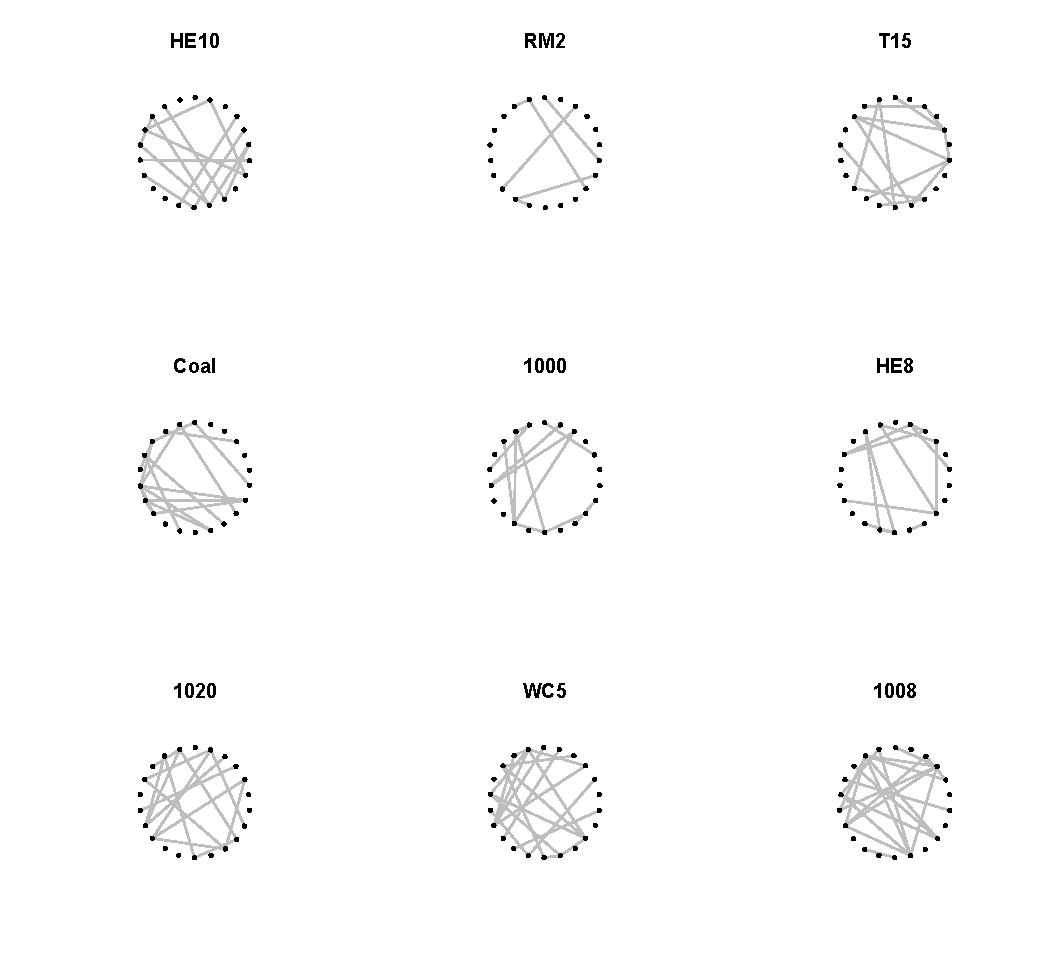
\includegraphics[width=15cm,height=14cm]{Fig1}
\caption{Community network graphs for different narrowleaf (\textit{Populus angustifolia}) genotypes in the Ogden Nature Center. Each node represents a species and a line between two points is a significant Kendall's correlation. The nodes are arrayed in the same position in the network graph for each genotype.}
\end{figure}

\end{document}  